%%%%%%%%%%%%%%%%%%%%%%%%%%%%%%%%%%%%%%%%%
% Stylish Article
% LaTeX Template
% Version 2.1 (1/10/15)
%
% This template has been downloaded from:
% http://www.LaTeXTemplates.com
%
% Original author:
% Mathias Legrand (legrand.mathias@gmail.com) 
% With extensive modifications by:
% Vel (vel@latextemplates.com)
%
% License:
% CC BY-NC-SA 3.0 (http://creativecommons.org/licenses/by-nc-sa/3.0/)
%
%%%%%%%%%%%%%%%%%%%%%%%%%%%%%%%%%%%%%%%%%

%----------------------------------------------------------------------------------------
%	PACKAGES AND OTHER DOCUMENT CONFIGURATIONS
%----------------------------------------------------------------------------------------

\documentclass[fleqn,10pt]{SelfArx} % Document font size and equations flushed left

\usepackage[english]{babel} % Specify a different language here - english by default

\usepackage{lipsum} % Required to insert dummy text. To be removed otherwise

\usepackage[defaultfam,light,tabular,lining]{montserrat} %% Option 'defaultfam'
%% only if the base font of the document is to be sans serig
\usepackage[T1]{fontenc}
\renewcommand*\oldstylenums[1]{{\fontfamily{Montserrat-TOsF}\selectfont #1}}
\renewcommand{\floatpagefraction}{.8} % for text coexisting with figs and tabs

\graphicspath{ {./images/} }

%----------------------------------------------------------------------------------------
%	COLUMNS
%----------------------------------------------------------------------------------------

\setlength{\columnsep}{0.55cm} % Distance between the two columns of text
\setlength{\fboxrule}{0.75pt} % Width of the border around the abstract

%----------------------------------------------------------------------------------------
%	COLORS
%----------------------------------------------------------------------------------------

\definecolor{color1}{RGB}{102, 102, 102} % Color of the article title and sections
%\definecolor{color1}{RGB}{178,34,34} % Color of the article title and sections
%\definecolor{color1}{RGB}{246,64,96} % Color of the article title and sections

%\definecolor{color2}{RGB}{0,20,20} % Color of the boxes behind the abstract and headings
\definecolor{color2}{RGB}{246,64,96}
%----------------------------------------------------------------------------------------
%	HYPERLINKS
%----------------------------------------------------------------------------------------

\usepackage{hyperref} % Required for hyperlinks
\hypersetup{hidelinks,colorlinks,breaklinks=true,urlcolor=color2,citecolor=color1,linkcolor=color1,bookmarksopen=false,pdftitle={Title},pdfauthor={Author}}

%----------------------------------------------------------------------------------------
%	ARTICLE INFORMATION
%----------------------------------------------------------------------------------------

\JournalInfo{
\includegraphics[scale=0.125]{NeoMeetup}}  
%Journal information
\Archive{ } % Additional notes (e.g. copyright, DOI, review/research article)

\PaperTitle{ArMeetup: blabla} % Article title

\Authors{Dario Bertazioli\textsuperscript{1}, Fabrizio D'Intinosante\textsuperscript{1}, Massimiliano Perletti\textsuperscript{1}*} % Authors
\affiliation{\textsuperscript{1}\textit{Data Science, Department of Computer Science, University of Milano Bicocca, Milan, Italy}} % Author affiliation
\affiliation{*\textbf{Corresponding author}: m.perletti@campus.unimib.it} % Corresponding author

\Keywords{Meetup --- ADD KEYWORDS--- Keyword3} % Keywords - if you don't want any simply remove all the text between the curly brackets
\newcommand{\keywordname}{Keywords} % Defines the keywords heading name

%----------------------------------------------------------------------------------------
%	ABSTRACT
%----------------------------------------------------------------------------------------

\Abstract{yolo}

%----------------------------------------------------------------------------------------

\begin{document}

\flushbottom % Makes all text pages the same height

\maketitle % Print the title and abstract box

\tableofcontents % Print the contents section

\thispagestyle{empty} % Removes page numbering from the first page

%----------------------------------------------------------------------------------------
%	ARTICLE CONTENTS
%----------------------------------------------------------------------------------------

\section*{Introduction}
{\small %small for text larger
\textbf{Meetup} è stato creato nel 2002 come piattaforma per mettere in contatto le persone nella vita reale. Fondato e guidato inizialmente da Scott Heiferman e Brendan McGovern, nel 2017 Meetup è stato acquisito da WeWork (ora The We Company). \\
Una volta completata la fase di registrazione, gli utenti possono: \\
\\
- Selezionare i propri interessi: ciò avviene sottoscrivendo dei topic precompilati dall'applicazione in modo da favorire il sistema di raccomandazione. Questi topic spaziano tra i più svariati ambiti, da quello professionale a quello degli hobby, fino ai più comuni, relativi ad eventi sociali. \\
\\
- Iscriversi a gruppi locali: una volta selezionati i topic di interesse il sistema di raccomandazione dell'applicazione suggerisce all'utente una serie di gruppi più o meno locali (a seconda dell'area di interesse selezionata dall'utente) che trattano i topic in oggetto o altri topic ad essi correlati. Ciò permette agli utenti di incontrare persone della propria zona che condividono le stesse passioni. Nel caso in cui tra i topic di interesse per l'utente ce ne siano alcuni che non trovano nessun riscontro in gruppi presenti sul territorio, l'applicazione suggerisce all'utente di creare lui stesso un gruppo con oggetto quel topic, consigliando di mettersi in contatto con altre persone che dimostrano quell'interesse, suggerendole attraverso il sistema di raccomandazione.\\
\\
- Partecipare ad eventi: i gruppi locali, nel corso del tempo, organizzano eventi, incontri, meeting con oggetto i topic dichiarati dai gruppi stessi. Una volta che un gruppo ha organizzato un evento l'utente può visualizzarli sulla propria home e, una volta visionati i dettagli, decidere di comunicare se partecipare oppure no e, nel caso volesse partecipare, se ha intenzione di portare degli ospiti, il tutto in maniera non vincolante. Inoltre, per non restringere troppo la sfera di interessi degli utenti, l'applicazione permette anche di selezionare diversi filtri per la home, tra cui uno apposito per visualizzare eventi organizzati da gruppi di cui non si fa parte o un filtro apposito per visualizzare gruppi di cui l'utente non è già membro e che magari non trattano topic per cui l'utente ha dichiarato interesse, ma che essendo pur sempre gruppi locali, l'utente potrebbe gradire o trovare interessanti.\\
\\
Il focus centrale dell'intero meccanismo dell'applicazione risulta quindi essere quello del "gruppo" visto come realtà associativa e fautore di momenti di aggregazione durante l'intero anno, molto spesso non guidati da una ristretta cerchia di capi ma, anzi, promotore di iniziative da parte dei suoi stessi membri. La varietà di gruppi, a seconda dei topic trattati, spazia tra:
\begin{enumerate}
\item Gruppi di socializzazione, che hanno come obiettivo principale quello di svolgere attività ludiche in compagnia, molto spesso anche promotori di veri e propri eventi di incontro per single.
\item Gruppi professionali, che si pongono l'obiettivo di mettere in contatto persone e professionisti di svariati campi attraverso workshop o presentazioni con il fine di fare crescere gli utenti dal punto di vista professionale.
\item Gruppi creativi, ovvero gruppi di progettazione e più vocati ad hobby ed alla pratica delle più svariate arti. \\
\end{enumerate}
Sintetizzando, quindi, la missione di Meetup è aiutare le persone a crescere e raggiungere i loro obiettivi attraverso connessioni autentiche e reali. Dal network professionale alla birra artigianale passando per workshop di programmazione, le persone usano Meetup per uscire dalla loro comfort zone, incontrare nuove persone, imparare cose nuove, perseguire le loro passioni e trovare sostegno in comunità che le aiutano a crescere.\\
Ad oggi, Meetup è disponibile in 186 Paesi, e conta più di 40 milioni di membri sulla piattaforma, con più di 320 mila gruppi attivi ed una media di 12 mila eventi al giorno.
}
%------------------------------------------------

\section{Goals}
{\small
Con l'analisi della rete sociale di Meetup e andando a studiare le relazioni che interconnettono le persone attraverso eventi sociali organizzati dai diversi gruppi presenti in tutto il globo, è possibile avere una mappatura più o meno dettagliata degli interessi comuni che portano ad agglomerare un significativo numero di soggetti instaurando relazioni tra di essi. \\
\\
Cercando di ricreare questa rete ci siamo posti alcuni obiettivi, considerando anche i limiti dovuti all'acquisizione dati, ovvero quella avvenuta in forma streaming:
\begin{itemize}
\item Effettuare misure quantitative semplici per verificare, banalmente, quali siano i paesi in cui la piattaforma è più utilizzata ed affermata;
\item Sfruttando le informazioni temporali, verificare quale sia il momento migliore della settimana e della giornata in cui organizzare un meetup per poter attrarre più persone possibili, considerando che la piattaforma è per lo più utilizzata per incontri di carattere professionale;
\item Sfruttando le informazioni spaziali, cercare di individuare quanto ampio sia il raggio di un evento in termini di attrazione degli utenti;
\item Utilizzando le informazioni relative ai topic trattati dai gruppi che organizzano gli eventi e ai topic che i membri dichiarano in sede di iscrizione alla piattaforma, valutare l'efficacia del sistema di raccomandazione della piattaforma, sempre considerando i limiti naturali imposti dallo streaming.
\end{itemize}
L'obiettivo del progetto, in sintesi, è quello di identificare correlazioni o tracce significative che possano determinare delle buone regole nella creazione di eventi di notevole impatto sociale; una piccola guida "\textbf{How to}" su come dev'essere organizzato un evento di successo.
}
%------------------------------------------------
\newpage
\section{Implementation: Architecture}
{\small %FIXME: IMPORTANT: da aggiungere caratteristiche quali tolerance failure et similia un po' ovunque
\subsection{Covered points}
L'intera strutturazione del progetto si pone come obiettivi didattici, oltre a quelli pratici già esposti, di coprire due delle tre \textbf{V} caratteristiche dei \textit{Big Data}:
\begin{enumerate}
\item \textbf{V}elocity: attraverso l'applicazione di raccolta dei dati provenienti da una fonte streaming, con tutte le problematiche a questa connessa, come connessione e immagazzinamento dei dati real time.
\item \textbf{V}olume: la raccolta dei dati ha prodotto un quantitativo di dati di notevole importanza, comportando la costruzione di un DB di dimensione superiore ai 2 GB. Ciò ha comportato la necessità di applicare tecniche e tool adeguati a compiere task su grandi moli di dati in tempi accettabili.
%\item \textbf{V}ariety: la raccolta dei dati non si è infatti limitata all'immagazzinamento tramite streaming, ma è stata applicata anche attraverso interrogazione a REST api necessitando, quindi, anche un lavoro a posteriori di riconduzione delle diverse fonti dei dati a formato comune con successivo instance matching, reso possibile dalla presenza di identificatori univoci presenti per ogni entità. 
\end{enumerate}
\subsection{Source}%WebSocket (RSVP) Rest API
Meetup, come già detto, mette a disposizione parte dei dati in suo possesso relativi a membri iscritti alla piattaforma, gruppi creati ed eventi organizzati nella stessa. In particolare, i dati sono forniti in due modalità: 

\paragraph{streaming data:} 
la piattaforma condivide dati in streaming, composti essenzialmente da \textbf{RSVP}.
Le RSVP sono risposte di feedback da parte degli utenti comunicanti agli organizzatori di un evento la loro partecipazione (o la loro non partecipazione, in quanto le risposte possono essere anche negative), all'evento stesso.
Un esempio di dato di questo genere è riportato sotto allo scopo di mostrarne la struttura.%FIXME: add fig.
%da fare un format migliore
\begin{itemize}[noitemsep]
\item \textbf{event}:
	\begin{itemize}[noitemsep]
	\item event\_id:	Unique alphanumeric identifier
	\item event\_name: Name of the event
	\item event\_url: URL to the full event page
	\item time: Event time if set in milliseconds since the epoch
	\end{itemize}
\item \textbf{group}:
	\begin{itemize}[noitemsep]
    \item group\_city: Group's home city
    \item group\_country: two-letter code of group's home country
    \item group\_id: Numeric identifier of the group
    \item group\_lat: Latitude of group's approximate location
    \item group\_lon: Longitude of group's approximate location
    \item group\_name: Name of the group
    \item group\_state: two-letter code of group's home state, if in US or CA
    \item group\_topics: Topics associated with this group
			\begin{itemize}[noitemsep]
			\item topic\_name: Longer name
        	\item urlkey: Unique keyword
			\end{itemize}
    \item group\_urlname: Unique portion of group's URL, no slashes
	\end{itemize}
\item guests: Number of guests the member is bringing
\item \textbf{member}: Member who RSVP'd
	\begin{itemize}[noitemsep]
    \item member\_id: Unique numeric id
    \item member\_name: Full name given
    \item other\_services: e.g. {"twitter": {"identifier": "MeetupAPI"}}
    \item photo: Thumbnail URL for member photo if one exists
	\end{itemize}
\item \textbf{mtime}: Last modified time of this RSVP, in milliseconds since the epoch
\item response: "yes" or "no"
\item rsvp\_id: Unique numeric identifier
\item \textbf{venue}: Venue, if public
	\begin{itemize}[noitemsep]
    \item lat: Latitude of the venue
    \item lon: Longitude of the venue
    \item venue\_id: Unique numeric identifier
    \item venue\_name
	\end{itemize}    
\end{itemize}
Abbiamo proceduto ad estrarre tali dati da websocket, sfruttando Nifi (vedasi prossimo paragrafo).
\paragraph{rest API:} Meetup permette anche un accesso piuttosto flessibile al database, esponendo tramite rest API informazioni riguardo a membri, gruppi ed eventi in formato JSON. Abbiamo sfruttato questa possibilità per arricchire i dati acquisiti in streaming: in particolare, abbiamo proceduto all'enrichment delle informazioni sui membri, integrando per ciascun membro:
\begin{itemize}[noitemsep]
\item la localizzazione spaziale, ovvero le coordinate geografiche (lat/lon) dichiarate in fase di registrazione così che il sistema di raccomandazione dell'applicazione possa suggerire gruppi su base geografica.
\item i topic in cui l'utente ha dichiarato di avere interesse al momento dell'iscrizione alla piattaforma, anche in questo caso per permettere al sistema di raccomandazione di suggerire gruppi per cui l'utente potrebbe avere interesse.
\end{itemize}
\subsection{Nifi}% Producer and blabla
\begin{figure}
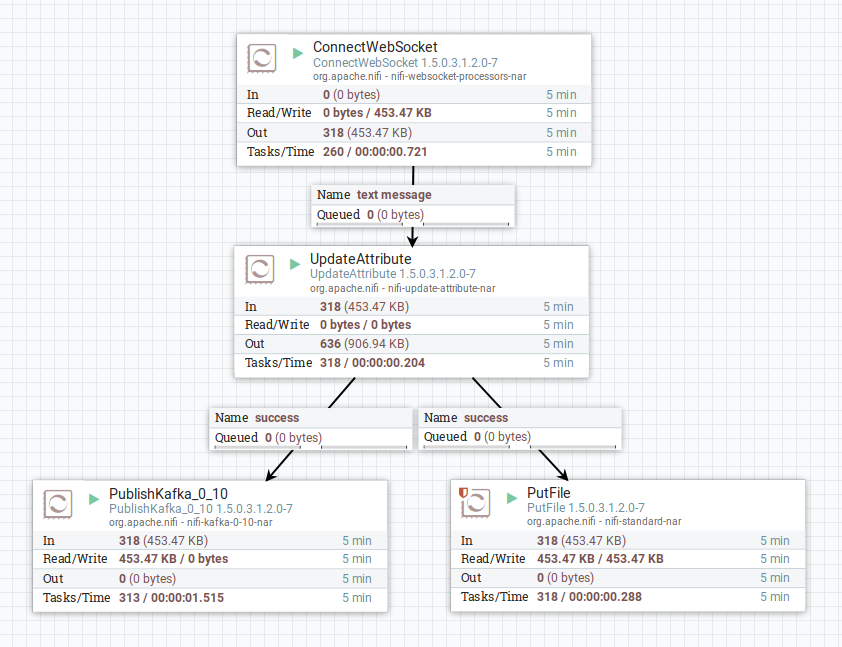
\includegraphics[scale=0.3]{images/nifi_workflow.png}
\caption{\label{nifi_workflow} Il workflow Nifi}
\end{figure}
Per acquisire i dati in streaming dalla piattaforma abbiamo implementato un workflow di Nifi (vedasi \textbf{fig.~\ref{nifi_workflow}}) contenente: 
\begin{itemize} %[noitemsep]
\item un nodo per la connessione alla \textbf{WebSocket} (\url{ws://stream.meetup.com/2/rsvps}, tramite un Client Jetty. 
\item un nodo per il parsing iniziale.
\item un nodo \textbf{PutFile}: abbiamo deciso di salvare i dati acquisiti su file system per due motivi principali: innanzitutto ciò è utile per avere una copia di backup dei dati, qual ora si verificassero problemi (ad esempio, con il corretto setting di \textit{retention time} di Kafka); in secondo luogo, terminato il periodo di acquisizione, per facilitare la copia dei dati su altre virtual machines, in modo da implementare contemporaneamente la stessa pipeline su più macchine, per poter confrontare (quantitativamente, in termini, ad esempio, di quantità di dati importati, tempi di esecuzione dei vari scripts etc.) i risultati ottenuti.
\item un nodo PublishKafka, comodo per effettuare l'ingestion dei dati in Kafka, configurandosi questo come un vero e proprio producer (vedasi sezione successiva). %FIXME: forse parentesi non necessaria
\end{itemize} 
I principali vantaggi che Nifi ci ha fornito sono la gestione facilitata della queue, la possibilità di parsing e la facile interfaccia con il Kafka Producer.
%Inoltre Nifi garantisce %FIXME: aggiungi fault tolerance etc dopo aver fatto check.
\subsection{Kafka} %Lambda Arch. and blabla
Considerata la natura dei dati a nostra disposizione, che ricordiamo consistere in un flusso di messaggi in streaming (RSVP), abbiamo deciso di fare un ingestion in Kafka, potendo successivamente esplorare, iterare, e preprocessare le informazioni tramite Python API.
Abbiamo inoltre modificato i parametri di RetentionTime, in modo tale che Kafka fungesse da primo storage temporaneo, in grado di salvare all'interno di un topic tutti i messaggi acquisiti in real time streaming, per poi poterli processare successivamente senza correre il rischio di perdere qualche informazione.
Come accennato, con l'API di Kafka per Python abbiamo potuto configurare un consumer per processare i dati, creando diversi \href{https://github.com/DBertazioli/Armeetup/tree/master/csv/struttura}{csv}, %(FIX: non saprei quanto entrare nei dettagli dei vari csv)
 in modo da facilitare e rendere più efficiente l'import nel database finale.
%(FIX: eventualmente accenna script per automatizzare)
\subsection{Neo4j}% Storing and querying
\begin{figure}
\centering
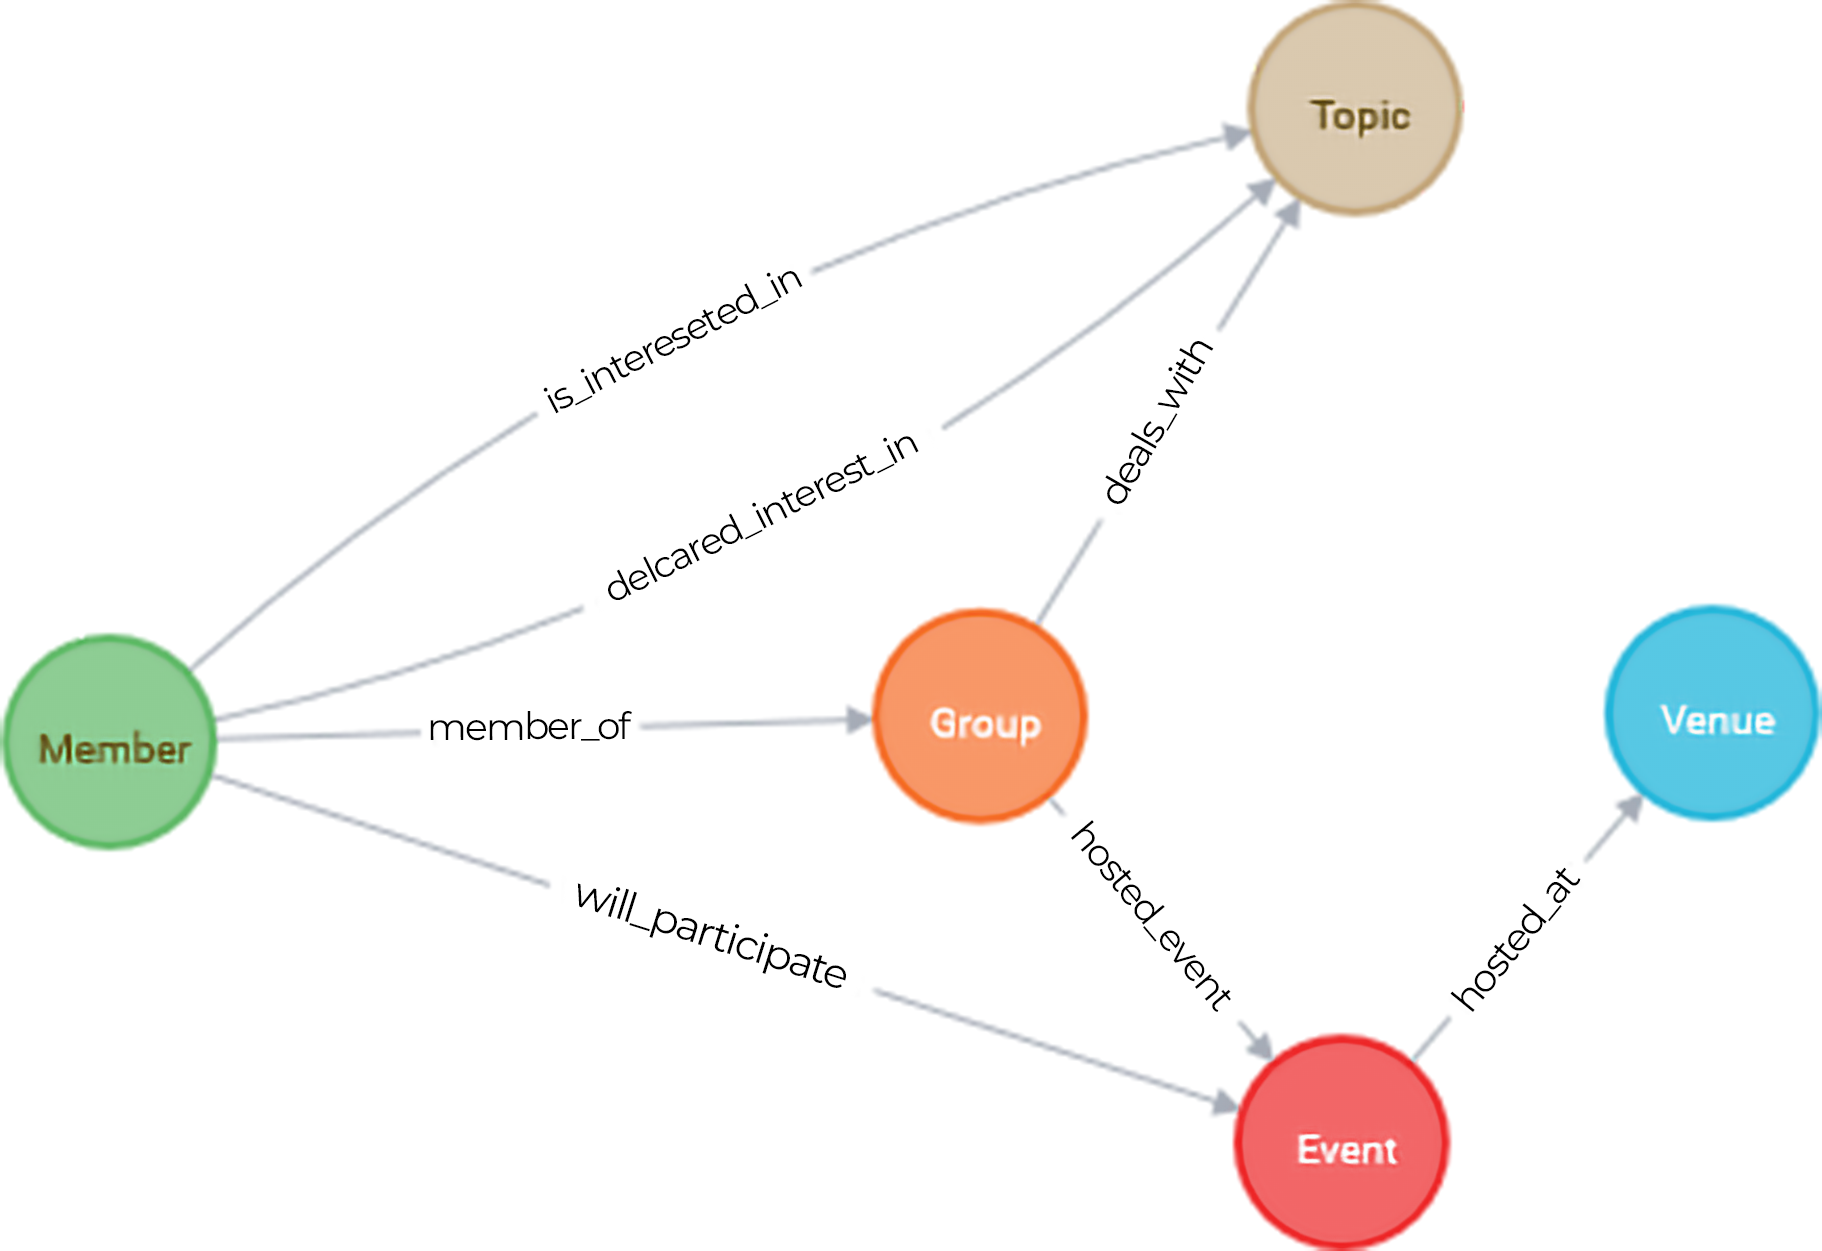
\includegraphics[scale=0.57]{graph.png}
\caption{\label{graph_neo4j} Schema graph DB}
\end{figure}
Abbiamo scelto inizialmente di salvare i nostri dati in un database a grafo per via della loro struttura naturale, che ben si presta ad essere schematizzata con nodi principali, proprietà e relazioni che interconnettono tali nodi. Abbiamo provveduto quindi all'import dei dati in Neo4j, sfruttando il linguaggio Cypher e l'ottimizzazione dell'import via csv, dopo aver in un primo momento tentato un approccio tramite l'api Python Py2Neo. Per facilitare un'eventuale serializzazione del processo di import, abbiamo creato uno script (Bash) che, una volta creati i csv, consente di automatizzare le varie chiamate alla cypher-shell, dato che il processo di creazione del database risulta piuttosto laborioso ma facilmente standardizzabile (\href{https://github.com/DBertazioli/NeoMeetup/blob/master/Scripts/import_cypher.sh}{import.sh}).
Questa soluzione però mal si prestava alla prospettiva di accumulare più dati, anche in vista di un possibile ampliamento degli orizzonti del progetto, dato che Neo4j non permette la distribuzione orizzontale dei propri database ma giova soltanto di una scalabilità di tipo verticale.
\subsection{ArangoDB}
Data a questo punto l'esigenza di trovare una soluzione che coniugasse il nostro bisogno di un database a grafo, ma che fosse anche in grado di essere scalabile orizzontalmente e quindi distribuibile con processi interni e non tramite segmentazione dei dati all'origine, anche nell'ottica di voler eventualmente implementare uno streaming continuo dall'RSVP API, abbiamo optato per ArangoDB, un DBMS multi-modello in grado di unire modelli documentale, a grafo e key-value con un solo linguaggio di programmazione. %nota riguardo la distribuzione del modello.
Sfruttando il particolare concetto di grafo nativo in ArangoDB abbiamo così realizzato una \textit{collection} per ogni vertice ed una \textit{edge-collection} per ogni arco del grafo.
Il database così realizzato presenta circa 1 milione e mezzo di singoli nodi e circa 28 milioni di relazioni tra questi, con un tempo di import su ArangoDB stimato in circa venti minuti.
}
\section{Results}
\paragraph{Misure quantitative semplici}:
%magari un grafico con relativo commento
\paragraph{Utilizzo delle informazioni temporali}:
Attingendo alle informazioni temporali degli eventi, presenti nei messaggi, ed applicando un'opportuna manipolazione per convertire l'originale formato timestamp in un formato umanamente più leggibile, siamo stati in grado di rispondere alla nostra seconda domanda di ricerca. Dopo aver infatti adattato i metadati temporali alle time zone così da avere una panoramica coerente sugli eventi Meetup tenutisi nel mondo, indipendentemente dal fuso orario, abbiamo provveduto a realizzare una tabella di Pivot, tenente conto della numerosità di partecipanti agli eventi discriminati per giorno della settimana e per fascia oraria della giornata. Una volta realizzata la tabella è stato quindi possibile procedere alla costruzione della \textit{heatmap} in \textbf{fig.~\ref{plot_heatmap}} 
per rappresentare al meglio queste informazioni. Appare infatti chiaro dalla visualizzazione come i momenti migliori della settimana per organizzare un evento risultino essere il Martedì, il Mercoledì ed il Giovedì nella fascia oraria 18.00/20.00 ed il Sabato mattina tra le 10.00 e le 12.00. Ciò si conforma bene alla nostra intuizione che la maggior parte dell'utenza di Meetup sembrerebbe essere rappresentata da lavoratori, professionisti, che sono quindi più propensi a partecipare ad eventi in orario non lavorativo o durante giorni non lavorativi.
\begin{figure}
\centering
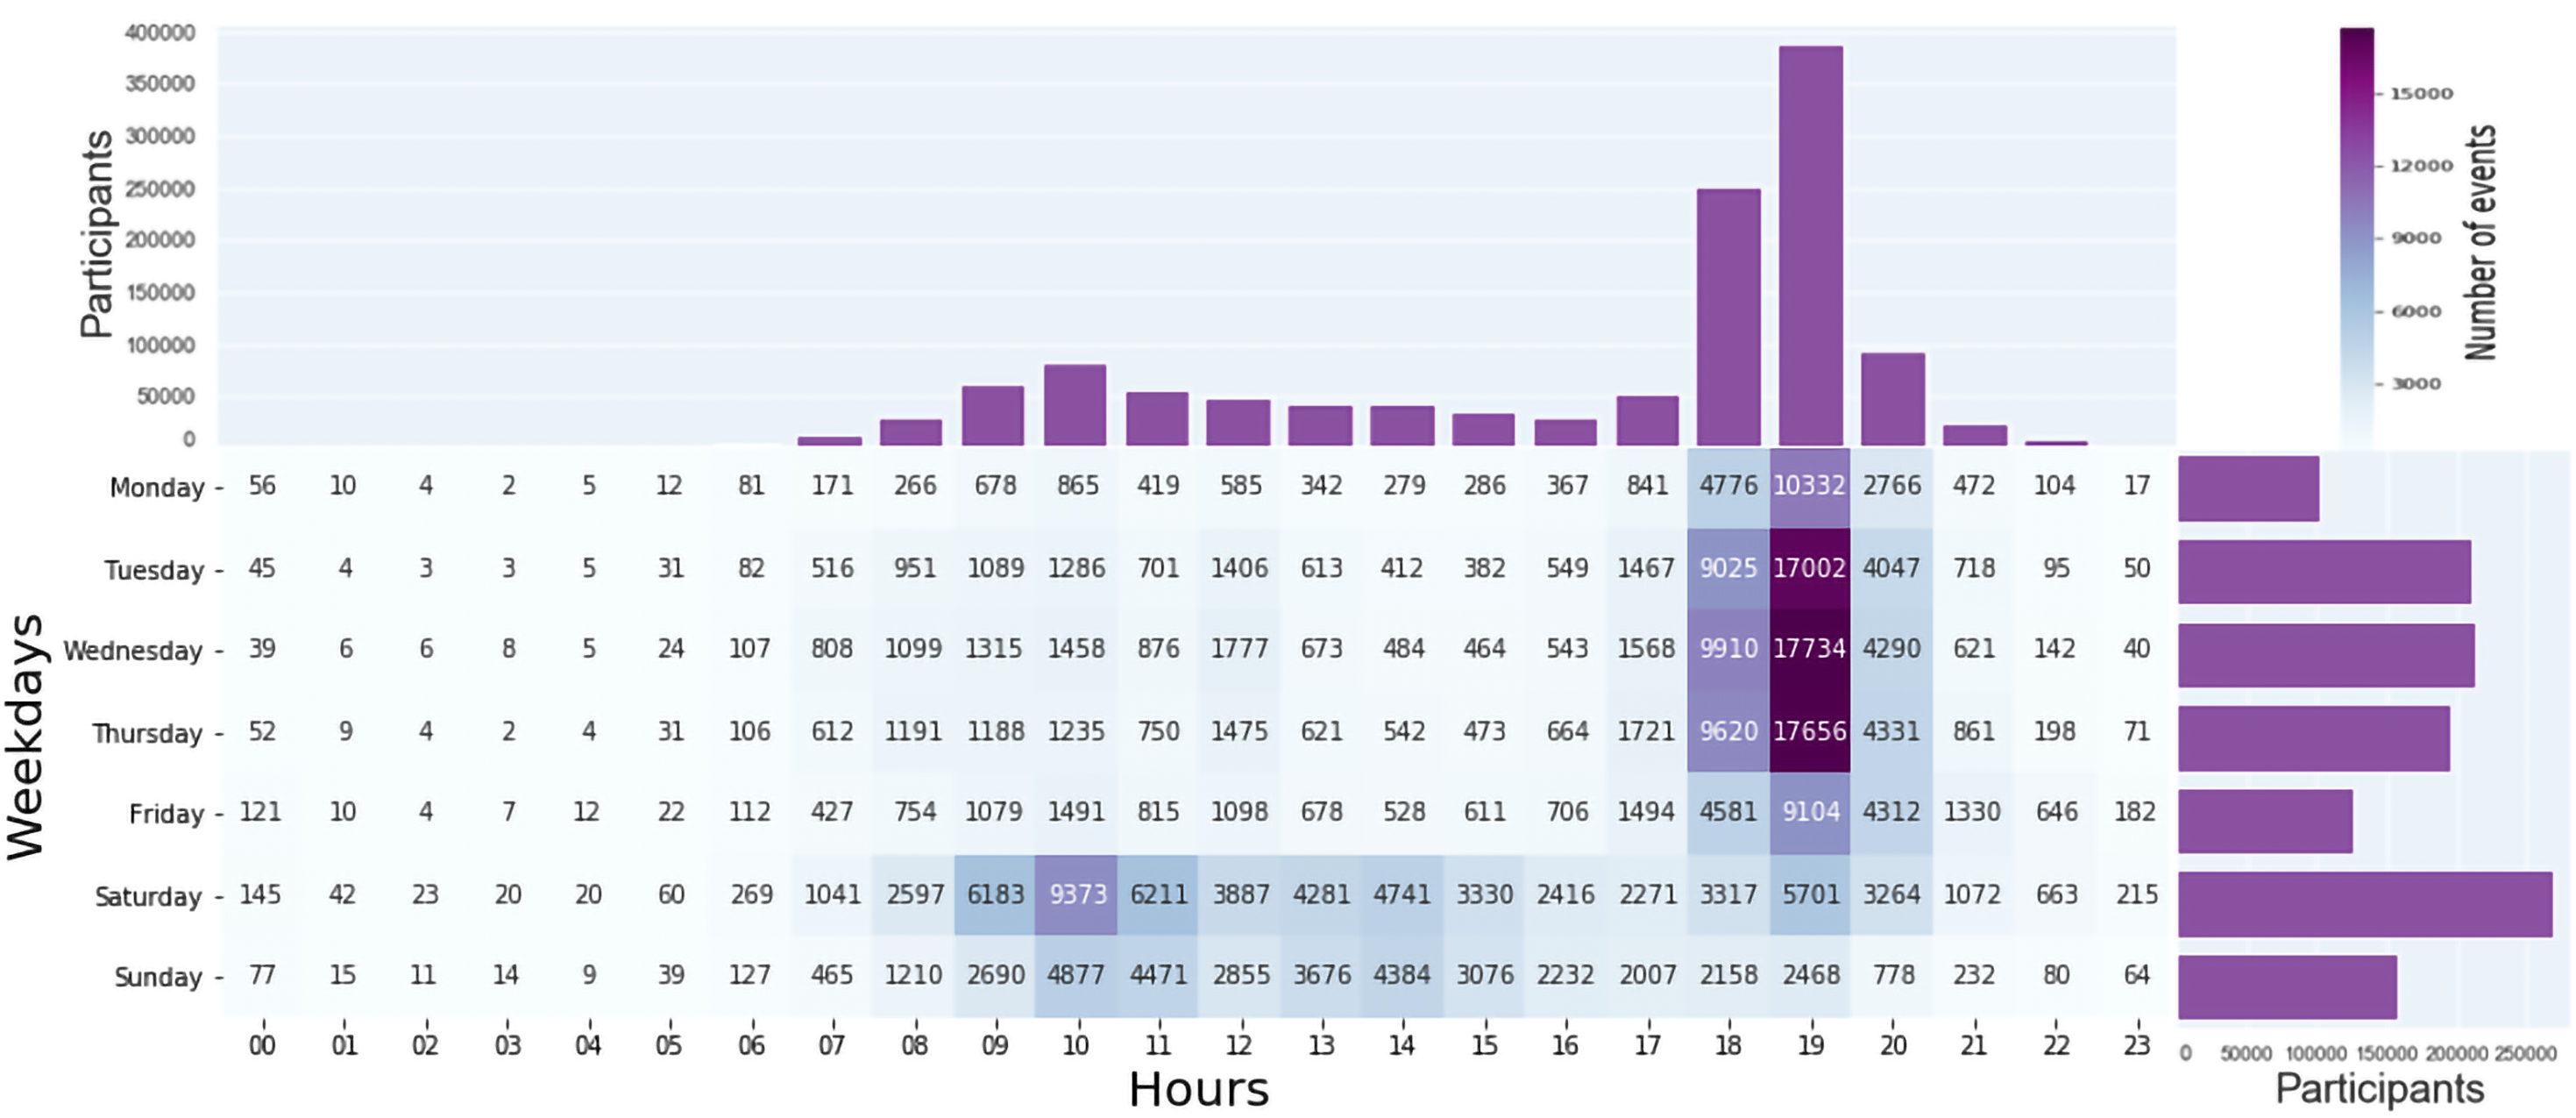
\includegraphics[width = 9.2 cm, height = 5 cm]{heatmap_with_barplot_v3.jpg}
\caption{\label{plot_heatmap} Heatmap distribuzione temporale degli eventi}
\end{figure}
\paragraph{Utilizzo delle informazioni spaziali}:
%riferimento a mappa interattiva con link
\paragraph{Valutazione efficacia sistema di raccomandazione}:
%distribuzione Jaccard similarity
%------------------------------------------------
\phantomsection
\section*{Interesting Challenges}
{\small
Durante la realizzazione del progetto abbiamo dovuto affrontare diverse problematiche legate ai più svariati ambiti, da quello della scalabilità in import dei dati a quello della velocità di processing.
\paragraph{Symbolic Links}: Avendo effettuato lo streaming utilizzando una sola Virtual Machine (VM), per poter trasferire i dati anche sulle altre macchine abbiamo provveduto a creare parallelamente all'ingestion diretta in Kafka anche un backup direttamente nella macchina. Ciò ci ha permesso di trasferire direttamente questo backup dalla macchina principale alle altre. Successivamente nelle nuove VM si rendeva quindi necessario implementare un ingestion dalla VM a Kafka per mezzo di un workflow Nifi, così da emulare la stessa procedura dello streaming. Per ovviare poi ad un bug/limite dei nodi \textit{getFile/FetchFile} di Nifi, che si verifica nel tentativo di eseguire un ingestion di elevata quantità di file in una sola volta, abbiamo escogitato una soluzione creando dei link simbolici, dividendo la creazione in sottocartelle, facendo così leggere al nodo \textit{GetFile} questi link e impostando il nodo in modo che venisse eliminato il link dopo la singola lettura/ingestion. Ciò ci ha permesso di conservare i dati originali ed impedire che i nodi di import li eliminassero, facendoci risparmiare tempo per quanto riguarda la creazione dei database di backup sulle diverse VM.
\paragraph{Ottimizzazione tempi di estrazione dei messaggi}:  \\ Con il fine di estrarre le singole entità presenti nei messaggi, che per la natura dello streaming risultavano ripetersi più volte a seconda delle interazioni degli utenti con il servizio, abbiamo tentato inizialmente un approccio mediante liste su python. Sinteticamente questo approccio consisteva nel creare un Kafka consumer tramite l'API kafka per python e, ciclando, produrre tutti i messaggi in nostro possesso estraendo le singole entità, come utenti, gruppi e altro, utilizzando due liste di cui una contenitore per le singole entità ed una come "black list" per tenere traccia delle entità già inserite e quindi da non riprocessare. Questo approccio si è però dimostrato limitato in termini di perfomance nel processare grandi volumi di dati e ci ha portati ad optare per una soluzione alternativa: utilizzando dei dizionari, e sfruttando gli ID presenti per ogni entità contenuta nei messaggi, abbiamo utilizzato questi ID come chiavi dei dizionari assegnandogli come valore tutte le proprietà associate a quell'entità. La differenza in termini di prestazioni si è dimostrata estremamente netta. Come si vede in \textbf{fig.~\ref{plot_lists_dicts}} la differenza è estremamente marcata, a partire dall'estrazione di più di 100 mila singole istanze il tempo richiesto dalle liste cresce esponenzialmente mentre quello dei dizionari resta sostanzialmente costante, per questo motivo per poter estrarre i CSV necessari all'import su Neo4j abbiamo deciso di adottare i dizionari.
\begin{figure}
\centering
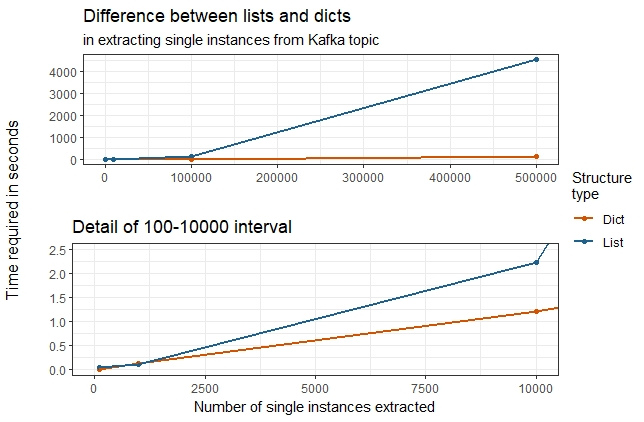
\includegraphics[scale=0.54]{viz_benchmark_lists_dicts.jpeg}
\caption{\label{plot_lists_dicts} Differenza di prestazioni fra liste e dizionari}
\end{figure}
\paragraph{Import Cypher vs Py2Neo}: Una volta ottenuti i CSV necessari all'import dei nodi e delle relazioni abbiamo innanzitutto tentato un approccio con l'API Py2Neo per python. Come per le liste in precedenza, l'API si è comportata bene sulle ridotte dimensioni, mentre al crescere del volume dei dati da importare si è resa inutilizzabile per gli elevati tempi d'attesa. Come si vede in \textbf{fig.~\ref{plot_cypher_py2neo}} l'import tramite cypher shell, meccanismo nativo di import per Neo4j, si dimostra fin dalle piccole dimensionalità molto più efficiente di Py2Neo mantenendo praticamente costante il tempo di import, con prestazioni che toccano circa i 12 secondi per importare 500 mila nodi distinti, contro i circa 80 minuti richiesti da Py2Neo.
\begin{figure}
\centering
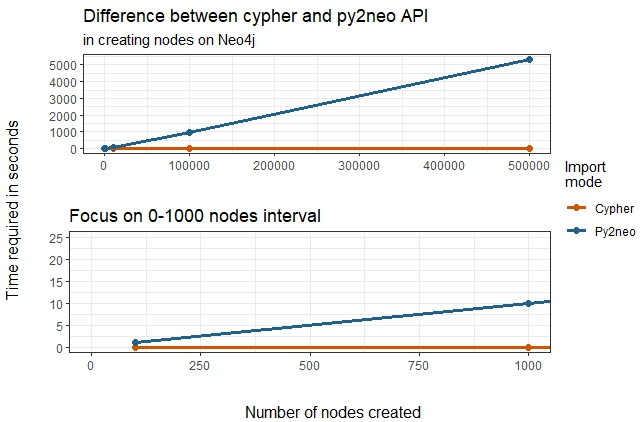
\includegraphics[scale=0.54]{viz_benchmark_cypher_py2neo.jpeg}
\caption{\label{plot_cypher_py2neo} Differenza di prestazioni fra Cypher e Py2Neo API}
\end{figure}
\paragraph{Cypher vs Arangoimp}
\begin{figure}
\centering
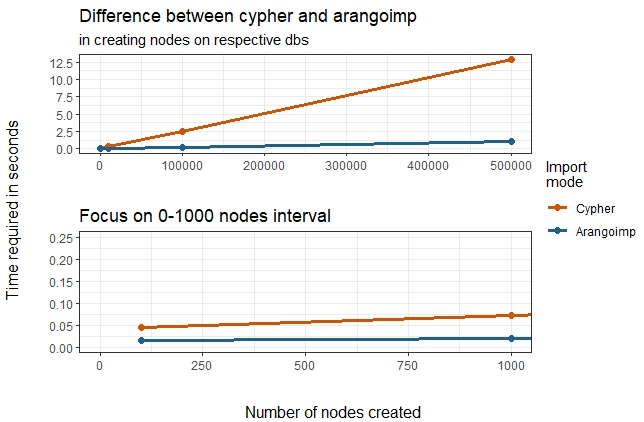
\includegraphics[scale=0.54]{viz_benchmark_cypher_arangoimp.jpeg}
\caption{\label{plot_cypher_arangoimp} Differenza di prestazioni fra Cypher e Arangoimp}
\end{figure}
Come si può vedere in \textbf{fig.~ \ref{plot_cypher_arangoimp}}
\paragraph{Scalability}: In prima istanza, dopo un primo streaming effettuato alla fine di dicembre 2018, abbiamo sfruttato questi dati per calibrare le nostre scelte in fatto di gestione dimensionalità. Questo primo streaming contava circa 1 milione di messaggi provenienti dall'API Meetup. Proprio grazie a questo quantitativo iniziale abbiamo potuto tarare le nostre decisioni su una dimensionalità realistica e già piuttosto complessa. Per questa ragione abbiamo deciso di sfruttare in prima istanza Kafka, che ha permesso di effettuare il primo storage senza essere condizionato in fase di consuming dalla dimensionalità dello storage stesso. Anche la scelta di un database a grafo, e nello specifico di Neo4j, è stata presa con l'intento di ottenere il massimo delle prestazioni possibili in fatto di scalabilità. Infine le scelte operate in fatto di processing dei dati con i dizionari per l'estrazione delle singole entità prima, e con la cypher shell per l'import di quelle entità su Neo4j dopo, si sono dimostrate essere vincenti per quello che è stato il vero e proprio streaming effettuato a febbraio 2019. Quest'ultimo infatti contava più di 2 milioni e mezzo di messaggi, con una dimensionalità finale del database di 1 milione e mezzo di singoli nodi e circa 28 milioni di relazioni tra questi.
\paragraph{Integrazione dei dati tramite rest API}: parallelizzazione e frequent throttlig. %Darito completa questo
\paragraph{Conversione dei metadati temporali}: Durante la fase di analisi dei dati con l'obiettivo di realizzare statistiche e visualizzazioni, ci siamo imbattuti nel problema della formattazione dei metadati temporali. Nello specifico tutti i metadati temporali provenienti dall'API di Meetup si presentano in formato timestamp in millisecondi con fuso orario UTC; questo rappresentava per noi un problema nella rappresentazione temporale degli eventi ad esempio, oppure per quella della sottoscrizione agli eventi da parte degli utenti. Per ovviare a questo inconveniente, e formattare questi metadati in formato date-time condizionati alle rispettive time-zone locali abbiamo sfruttato i metadati riguardanti la localizzazione degli utenti al momento della sottoscrizione agli eventi e, quindi, alla generazione del messaggio RSVP. Partendo quindi da queste informazioni in formato latitudine/longitudine abbiamo innanzitutto localizzato le corrispondenti time-zone attraverso la libreria \textit{timezonefinder} per python e, successivamente, attraverso la libreria \textit{pytz} abbiamo potuto convertire i timestamp in date-time condizionatamente alla time-zone prima definita. Lo sviluppo dei dati è visibile in \textbf{fig.~\ref{datetime_timezoned}}, dove è possibile visualizzare come il dataset si sia trasformato durante i passaggi descritti.
\begin{figure}
\centering
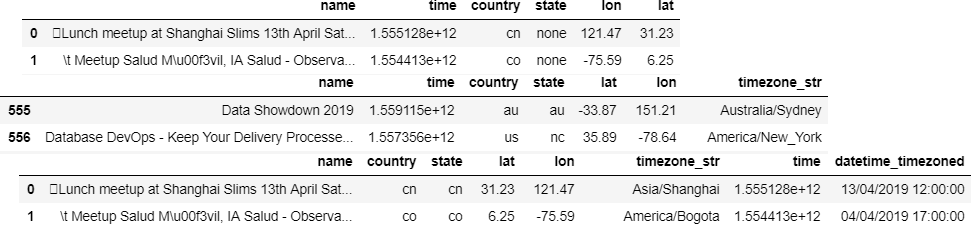
\includegraphics[width = 9 cm, height = 3.5 cm]{datetime_timezoned.png}
\caption{\label{datetime_timezoned} Passaggi conversione timestamp into datetime timezoned}
\end{figure}
}
\section*{Acknowledgments} % The \section*{} command stops section numbering

\addcontentsline{toc}{section}{Acknowledgments} % Adds this section to the table of contents

So long and thanks for all the fish.

%----------------------------------------------------------------------------------------
%	REFERENCE LIST
%----------------------------------------------------------------------------------------
\phantomsection
\bibliographystyle{unsrt}
\bibliography{sample}

%----------------------------------------------------------------------------------------

\end{document}